\section{Introduction}

Dans ce chapitre, nous détaillons l’analyse et la spécification des besoins fonctionnels et non fonctionnels de l’application \textit{JourneyBuddy}.  
Nous avons choisi la méthodologie agile SCRUM comme démarche de gestion de projet, favorisant un développement itératif et incrémental.  
Ce chapitre présente d'abord les exigences à satisfaire, puis l’environnement de travail retenu ainsi que les architectures générales adoptées (système et applicative).  
Enfin, nous clôturons par la planification générale de notre sprint, incluant les priorités, risques, et cas d’utilisation globaux.

\section{Analyse des besoins}

\subsection{Identification des besoins fonctionnels}

L’application est destinée à des voyageurs qui souhaitent planifier des itinéraires complets à l’aide d’une intelligence artificielle, incluant la réservation de vols, d’hôtels et d’activités touristiques.  
Les besoins fonctionnels définissent les fonctionnalités principales à implémenter telles que :

\begin{itemize}
    \item Création et gestion de compte utilisateur.
    \item Planification de voyage multi-étapes.
    \item Recherche intelligente de vols, hôtels et activités.
    \item Suggestions automatiques basées sur les préférences.
    \item Visualisation d’itinéraires.
\end{itemize}

\subsection{Identification des besoins non fonctionnels}

Les exigences non fonctionnelles portent sur :

\begin{itemize}
    \item \textbf{Performance} : temps de réponse acceptable même en cas de forte charge.
    \item \textbf{Sécurité} : protection des données utilisateurs (authentification, HTTPS...).
    \item \textbf{Accessibilité} : compatibilité multiplateforme via React Native.
    \item \textbf{Scalabilité} : architecture permettant l’extension future des services.
\end{itemize}

\section{Planification du traitement des cas d'utilisation}

Nous avons planifié les différentes fonctionnalités à travers un backlog produit en lien avec les cas d’utilisation, en tenant compte des priorités et des risques potentiels.

\subsection{Priorité}

\begin{itemize}
    \item \textbf{Haute} : fonctionnalités essentielles au fonctionnement de base.
    \item \textbf{Moyenne} : fonctionnalités utiles mais non critiques.
    \item \textbf{Basse} : compatibilité multiplateforme via React Native.
    \item \textbf{Scalabilité} : ajouts secondaires ou esthétiques.
\end{itemize}

\subsection{Risques}

Certains éléments du projet présentent des risques potentiels à anticiper :

\begin{itemize}
    \item Dépendance à des API externes (fluctuations, indisponibilité).
    \item Volume de données à gérer en base.
    \item Complexité de l’algorithme de recommandation.
\end{itemize}

\subsection{Diagramme de cas d'utilisation globale}

\begin{figure}[H]
    \centering
    \includegraphics[width=0.9\textwidth]{usecases/usecase}
    \caption{Diagramme de cas d'utilisation global de JourneyBuddy}
\end{figure}

\section{Description de l'application}

L’application \textbf{JourneyBuddy} est une application mobile construite avec la stack \textbf{MERN} :

\begin{itemize}
    \item \textbf{Frontend} en React Native, pour développer une interface utilisateur native sur iOS et Android.
    \item \textbf{Backend} en Node.js et Express.js, pour gérer la logique métier et les routes.
    \item \textbf{Base de données} MongoDB, orientée documents, idéale pour stocker des données flexibles et évolutives.
\end{itemize}

\subsection{Environnement de Travail}

Le projet adopte la stack MERN, qui combine MongoDB, Express, React Native et Node.js. Cette architecture permet un développement complet (frontend + backend) en JavaScript, favorisant la rapidité et la cohérence.

\begin{figure}[H]
    \centering
    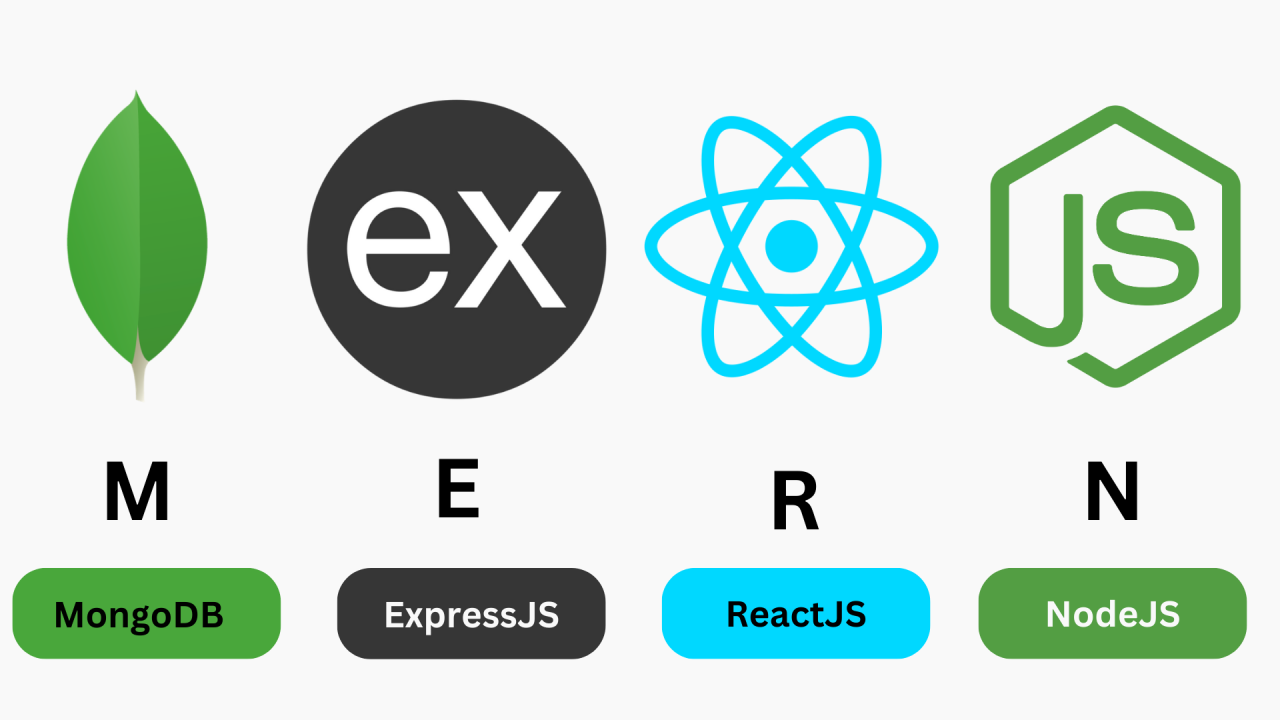
\includegraphics[width=0.7\textwidth]{logos/mern.png}
    \caption{Architecture MERN choisie}
\end{figure}

\renewcommand{\thesubsubsection}{\thesubsection.\arabic{subsubsection}} % Active la numérotation des subsubsection

\subsubsection{1. Outils de Développement et Modélisation}

\begin{itemize}
    \item \textbf{Visual Studio Code} : éditeur principal pour le développement de code.
    \begin{figure}[H]
        \centering
        
\includegraphics[width=0.5\textwidth]{logos/vscode.png}
        \caption{Environnement de développement : VS Code}
    \end{figure}

    \item \textbf{Visual Paradigm} : outil de modélisation UML et de conception visuelle utilisé pour l’analyse, la conception et la documentation des systèmes logiciels.
    \begin{figure}[H]
        \centering
        
\includegraphics[width=0.5\textwidth]{logos/visualparadigm.png}
        \caption{Outil de modélisation : Visual Paradigm}
    \end{figure}

    \item \textbf{Docker} : plateforme de conteneurisation permettant d’empaqueter des applications et leurs dépendances dans des conteneurs légers, portables et reproductibles.
    \begin{figure}[H]
        \centering
        
\includegraphics[width=0.3\textwidth]{logos/docker.png}
        \caption{Docker - Conteneurisation et virtualisation légère}
    \end{figure}

    \item \textbf{Docker Hub} : registre public officiel de Docker, permettant d’héberger, de partager et de télécharger des images de conteneurs.
    \begin{figure}[H]
        \centering
        
\includegraphics[width=0.3\textwidth]{logos/dockerhub.png}
        \caption{Docker Hub - Registre d’images de conteneurs}
    \end{figure}
\end{itemize}

\subsubsection{2. Plateforme de Développement}

\begin{itemize}
    \item \textbf{MongoDB Atlas} : base de données cloud sécurisée pour héberger les données.
    \begin{figure}[H]
        \centering
        
\includegraphics[width=0.5\textwidth]{logos/mongodb-atlas.png}
        \caption{MongoDB Atlas - Plateforme de base de données cloud}
    \end{figure}

    \item \textbf{MongoDB Compass} : interface graphique pour la visualisation et la manipulation des collections MongoDB.
    \begin{figure}[H]
        \centering
        
\includegraphics[width=0.7\textwidth]{logos/mongodb-compass.png}
        \caption{MongoDB Compass - Outil de gestion des collections}
    \end{figure}
\end{itemize}

\subsubsection{3. Frameworks Utilisés}

\paragraph{React Native} est un framework open-source développé par Meta permettant de créer des applications mobiles natives en JavaScript, facilitant ainsi le développement multiplateforme.

\begin{figure}[H]
    \centering
    
\includegraphics[width=0.3\textwidth]{logos/react-native.png}
    \caption{Framework React Native}
\end{figure}

\textbf{Avantages de React Native :}
\begin{itemize}
    \item Code partagé entre iOS et Android.
    \item Large communauté active et support continu.
    \item Performances proches du natif.
    \item Intégration aisée avec des API tierces.
\end{itemize}

\paragraph{Node.js et Express} forment un duo performant pour créer une API RESTful efficace. Node.js offre un environnement d'exécution côté serveur, tandis qu'Express fournit une structure légère pour la gestion des routes et des middlewares.

\begin{figure}[H]
    \centering
    
\includegraphics[width=0.25\textwidth]{logos/nodejs.png}
    \hspace{0.05\textwidth}
    
\includegraphics[width=0.25\textwidth]{logos/express.png}
    \caption{Node.js (à gauche) et Express (à droite)}
\end{figure}

\subsubsection{4. Langages Utilisés}

\begin{itemize}
    \item \textbf{TypeScript} : surensemble typé de JavaScript permettant de détecter les erreurs à la compilation.
    \begin{figure}[H]
        \centering
        \includegraphics[width=0.25\textwidth]{logos/typescript.png}
        \caption{Langage TypeScript}
    \end{figure}
\end{itemize}

\section{Architecture Adoptée}

L’architecture choisie définit la structure logicielle du système, garantissant modularité, maintenabilité et évolutivité.

\subsection{Architecture Système}
\setcounter{secnumdepth}{3}
% \hspace{0.2cm}
\subsubsection{Architecture 2-Tiers}
\setcounter{secnumdepth}{3}

L'architecture 2-Tiers repose sur une structure client-serveur classique, dans laquelle l'interface utilisateur (client) communique directement avec le serveur de base de données. Ce modèle est simple à implémenter et adapté aux applications légères, mais il présente des limitations en termes de scalabilité et de séparation des responsabilités.

\begin{figure}[H]
    \centering
    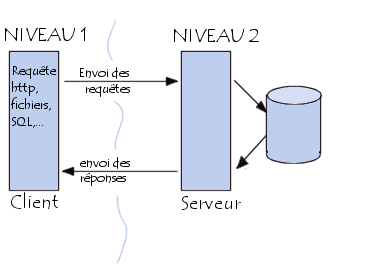
\includegraphics[height=0.4\textheight, width=0.7\textwidth]{figures/2-tier.png}
    \caption{Architecture 2-Tiers : client-serveur}
\end{figure}

\subsubsection{Architecture N-Tiers}

L'architecture N-Tiers introduit plusieurs couches logiques (présentation, logique métier, accès aux données, etc.), chacune jouant un rôle distinct. Cette séparation améliore la modularité, la sécurité et la maintenabilité, en facilitant les tests et l’évolution du système. Elle est particulièrement adaptée aux applications complexes à fort volume de données.

\begin{figure}[H]
    \centering
    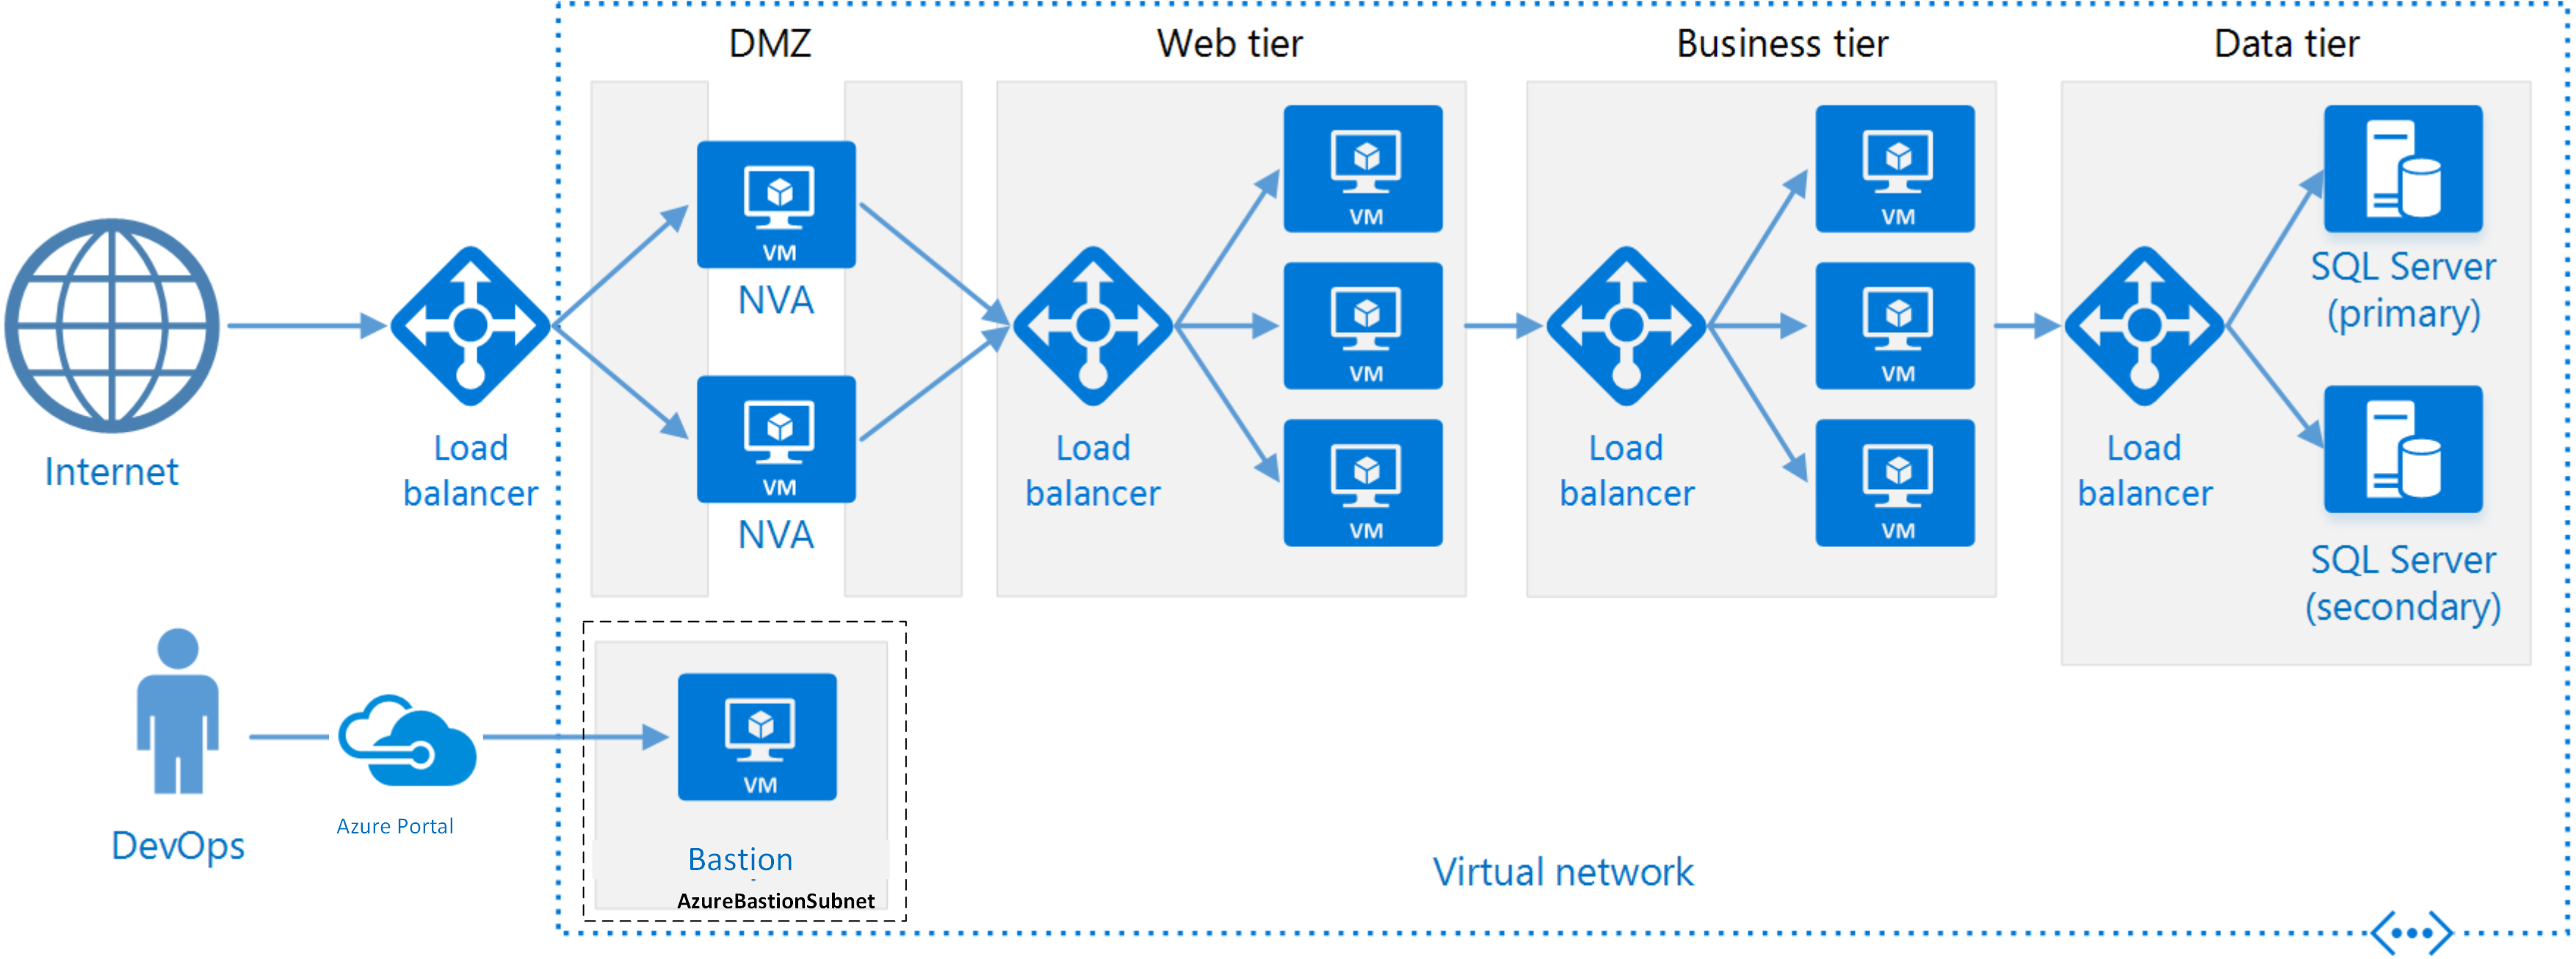
\includegraphics[height=0.4\textheight, width=0.9\textwidth]{figures/n-tier-arch.png}
    \caption{Architecture N-Tiers avec séparation logique en couches}
\end{figure}

\subsubsection{Architecture Adoptée : 3-Tiers}

JourneyBuddy adopte une architecture 3-Tiers, qui constitue une forme spécialisée de l’architecture N-Tiers. Elle se compose de trois couches principales :
\begin{itemize}
    \item \textbf{La couche présentation (frontend)} : gérée via React Native, elle gère les interfaces utilisateurs.
    \item \textbf{La couche logique métier (backend)} : assurée par Node.js et Express, elle traite les règles métiers et les requêtes.
    \item \textbf{La couche données} : gérée par MongoDB, elle stocke et fournit les informations.
\end{itemize}
Cette approche offre un excellent équilibre entre complexité, performance et évolutivité.

\newpage
\begin{figure}[H]
    \centering
    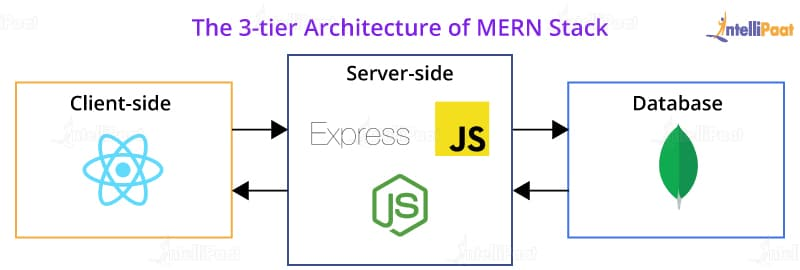
\includegraphics[width=0.8\textwidth]{figures/The-3-tier-Architecture-of-MERN-Stack.png}
    \caption{Architecture 3-Tiers retenue pour JourneyBuddy}
\end{figure}

\subsection{Architecture de l’application}

L'application suit le modèle MVC (Modèle – Vue – Contrôleur), une architecture classique permettant de séparer la gestion des données, la logique métier et l’affichage utilisateur.

\begin{itemize}
    \item \textbf{Modèle (Model)} : gère les données de l'application ainsi que les règles métiers. Il interagit directement avec la base de données.
    \item \textbf{Vue (View)} : représente l'interface utilisateur. Elle affiche les données provenant du modèle et transmet les interactions utilisateur au contrôleur.
    \item \textbf{Contrôleur (Controller)} : fait le lien entre le modèle et la vue. Il traite les entrées utilisateur et met à jour les données en conséquence.
\end{itemize}

\begin{figure}[H]
    \centering
    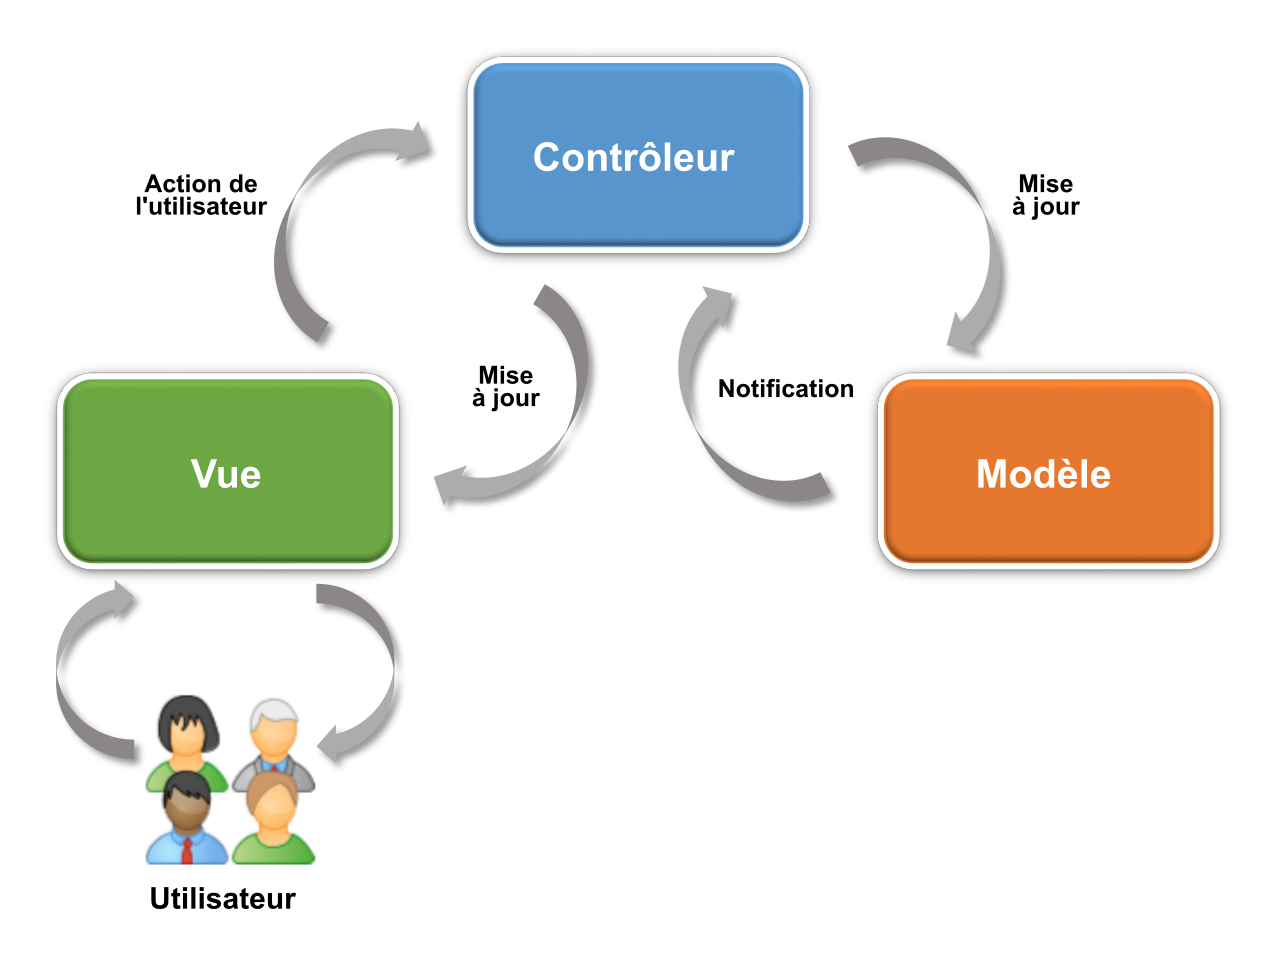
\includegraphics[width=\textwidth, height=0.3\textheight, keepaspectratio]{logos/mvc.png}
    \caption{Architecture de l'application JourneyBuddy (MVC)}
\end{figure}

\section{Conclusion}

L'analyse détaillée du projet JourneyBuddy a permis de définir les besoins fondamentaux, l’architecture technique, les outils à employer et les méthodes agiles à mettre en place. La combinaison de la stack MERN, de l’approche MVC, et de la gestion Scrum garantit une base solide pour assurer la réussite de l’application mobile.
